\section{Path Management}
\label{sec:path-management}

%\begin{figure}[htbp]
%	\centering
%		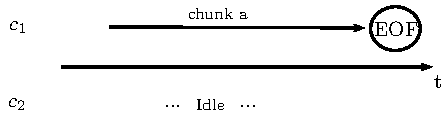
\includegraphics[width=\linewidth]{Figures/path-manager-why-1.pdf}
%		\rule{35em}{0.5pt}
%	\caption[Bad Path Management Scenario]{Bad Path Management: Assuming $c_2$ has a higher throughput than $c_1$, here the better path has idle time due to a bad initial path choice.}
%	\label{fig:bad-path-management-1}
%\end{figure}

The path management determines which end-points to use for a new connection, meaning which client interface and server IP are used to establish a new path. 

In our current approach we define one interface as primary, meaning that this interface will always be used to open the first path to a new server. 
Especially in mobile environments it makes sense to prefer a certain interface such as \wifi, since an \lte~interface might introduce additional economical cost to the user. 

In general, the first request to a new domain is sent over the primary interface and after receiving the response from the server, including the object's actual size, the path manager decides whether it is worth opening a new path. 
In case a second path is needed, we use the second interface to establish a connection. 
Note, that in case of web page downloads most embedded objects are usually downloaded from the same domain. 
Consequently, already opened paths from a previous object download can be reused when requesting another object from the same domain. 
When reusing paths, we always select the in terms of throughput best idle path to start a new request, hence the primary interface might not be chosen first in subsequent requests.

%Further we start work on a second approach we call 2-initial-path mechanism. 
%This mechanism initially and simultaneously opens 2 paths requesting two consecutive chunks of an initial chunk size without knowing the actual file size yet. 
%We expect a great speedup during the initial phase. 
%Still a problem arises if the requested object is of less size than the initial chunk size, meaning that the second request is an out of range request, which will result in an error response by the server. 
%Currently we focus on objects of size bigger than the initial chunk size. 
%Dealing with objects that are smaller than the initial chunk size is part of future work.
